\documentclass[conference]{IEEEtran}
\ifCLASSINFOpdf
\else
\fi
\usepackage{graphicx}
\usepackage{amssymb,amsmath,bm}
\usepackage{textcomp}
\usepackage{verbatim} 
\def\vec#1{\ensuremath{\bm{{#1}}}}
\def\mat#1{\vec{#1}}

\begin{document}

\title{Group Delay Functions for Speaker Diarization}

\author{
\IEEEauthorblockN{{ Mohit Yadav, Anil K Sao, A D Dileep and Padmanabhan Rajan}\\
Indian Institute of Technology Mandi, India\\ 
\  {\small \tt mohit\_yadav@students.iitmandi.ac.in \& \{anil, addileep and padman\}@iitmandi.ac.in}
}
}

\maketitle


\begin{abstract}

Speaker Diarization is the task of determining {\bf\textit{``who spoke when"}} in a speech recording of an unknown duration that contains an unknown number of speakers. The very unsupervised nature of this task makes it more challenging and demanding for the used features to be highly discriminative across speakers. Popularly used spectrum-related features for speaker diarization take into account merely the magnitude information and do not utilize information embedded in phase due to the complications involved its processing. However, the information contained in phase has been shown beneficial for (mostly supervised) speech tasks, now it is being explored for speaker diarization. In this work, we propose group-delay functions based features for speaker diarization. Group-delay functions are the representations of phase of Fourier spectrum, which overcomes the issues in processing the phase. We present our results on a publicly available meeting corpus. Our experiments demonstrate that the features derived from group-delay functions provide comparable or improved diraization accuracy over and on fusion with the popularly used mel-frequency cepstrum coefficients (MFCC) features. \\

\end{abstract}
\IEEEpeerreviewmaketitle

%\noindent{\bf Index Terms}: Speaker diarization, group-delay functions, all-pole model, agglomerative information-bottleneck.


\section{Introduction}
\label{intro}

A notable development in processing power has made digitization of large volumes of spoken documents like broadcast, meeting, lecture room conversations \cite{reviewPaper2,reviewPaper3}. With this digitization, the utility of speaker diarization systems has increased tremendously \cite{reviewPaper1,reviewPaper4}, and the result is a large number of speech applications utilizing speaker diarization systems such as information retrieval, speech and speaker indexing, document content structuring, speaker recognition in presence of multiple or competing speakers and to help in speech-to-text transcription. Two popular approaches for speaker diarization are based on HMM-GMM \cite{reviewPaper1} and the information-bottleneck(IB) principle \cite{aIB2}. The latter approach presents a non-parametric solution and has computational advantages over the earlier approach. Therefore, we focus on the diarization system based on the latter approach.  

%\subsection{Related Work}
In recent years, the scientific community has seen significant amount of work on improving features for diarization systems. Broadly this work can be divided into three categories based on the focus of work, namely, spatial information fusion, robust overlapped speech handling and learning-based features. Spatial information fusion based methods exploit the multiple recordings acquired from various channels of a microphone array to obtain a robust feature representation \cite{aIB3,aIB4,featAngle,speakerUPM,featSpatial,MDM}. These methods enjoy the resultant spatial redundancy and claim to provide complementary features to conventionally used MFCC features \cite{MDM}. On the other hand, rest of the categories do not make any explicit use of spatial information arising due to multiple recordings, rather, make use of single enhanced recording obtained after beamforming all available recordings \cite{beamforming}. 

Next category of methods are motivated by fact that the effective handling of overlapped speech is considered to be at the limits of the current state of the art of speaker diarization systems \cite{reviewPaper1,featOverLap}. In the same spirit, authors in \cite{featProsody,featOverLap} have explored long-term conversational and prosodic features to detect and handle overlapped speech more robustly. Authors in \cite{featSC} have also shown improvements by deriving features from representation obtained using convolutive non-negative sparse-coding. and the last category of methods advocate the use of features obtained by applying learning-based methods. Authors in \cite{featANN}, have proposed an artificial-neural-network based method to learn a feature transform, aimed to distinguish segments from different speakers. Similarly, authors in \cite{featPCAnLDA} utilize traditionally used principal-component-analysis and linear-discriminant-analysis to perform feature selection, both at the initial and the final stages of diarization system respectively. With an exception to above mentioned categories, authors in \cite{featFilterBank}, have applied features derived using filter-bank-slope of magnitude spectrum for speaker diarization, and attributed their success to their ability to emphasize formants. 

Feature derived from magnitude such as MFCC are ubiquitously used in various speech tasks. On the other hand, use of phase of short-term spectrum is not so spread widely, due to additional involved difficulties in their processing. However, there has been a significant increase in interest to utilize information from phase of short-term Fourier spectrum recently \cite{phaseImportantInterspeech14,gdSurvey}. {\textit{Group delay functions}} and its variants have been proposed to mitigate difficulties involved in processing of the phase of the short-term spectrum. Features derived from group-delay functions have shown promise for other speech tasks, and it is now explored for speaker diarization \cite{modifiedGD,allPoleGdSid}. 

In this work, we propose to derive features from group-delay functions for information-bottleneck based speaker diarization system. The primary objective of this work is to demonstrate whether group-delay based features are capable of capturing speaker information independently or in context of (an unsupervised task) speaker diarization and introduce improvement in the results with or without fusion with the existing features. 

The remainder of this paper is organized as follows: Section \ref{fe} presents group delay functions and briefly discusses difficulties involved in its processing. Subsequently, Section \ref{system} introduces IB based diarization (used in our experiments), performed feature analysis of group delay based function in context of used system, and fusion with MFCC. In Section \ref{experimentsNresults}, we evaluate and discuss the performance of group delay-based features for the introduced system on AMI dataset \cite{AMIData}. Lastly, Section \ref{conclude} provides conclusion and future work directions.    

\section{Group delay functions}
\label{fe}
Let us denote a frame of speech as $x(n)$ and its Fourier transform as $X(\omega)$. The polar representation of $X(\omega)$ can be written as follows:

\begin{equation}
X(\omega) = |X(\omega)| e^{j\theta(\omega)} 
\label{equ:FT}
\end{equation}     
where $|X(\omega)|$ and $\theta(\omega)$ refers to magnitude and phase part of the spectrum respectively. And the group-delay function is defined as the negative derivative of unwrapped phase of Fourier transform, and can be written as follows: 
\begin{equation}
\tau(\omega) =  - \frac{d}{d\omega} \theta(\omega)
\label{equ:GDF_def}
\end{equation}

Multiplication in magnitude domain results in an addition in group-delay domain, hence smaller influence by other peaks in proximity. Due to this property, group-delay functions achieves higher resolution as clearly evident in (bottom panel of the) Fig.\ref{fig:all-pole}. Even very closely spaced (anti)resonance peaks are better resolved in group-delay domain and confines resonance information to narrow regions around the zero or pole location. The above mentioned properties of group-delay functions makes them attractive to derive features. However, computation of unwrapped phase of Fourier transform is a non-trivial task. One method which bypasses the issues of phase unwrapping by using the following expression to compute group-delay function directly (also detailed in \cite{gdSurvey}) :

\begin{equation}
\tau(\omega) = \frac{X_R(\omega)Y_R(\omega) + X_I(\omega)Y_I(\omega)}{|X(\omega)|^{2}}
\label{eq:GDF_com}
\end{equation}

where $X(\omega)$ and $Y(\omega)$ are the Fourier transforms of speech signal $X[n]$ and $Y[n] = nX[n]$. $|X(\omega)|$ represents magnitude of Fourier transform. Subscripts $R$ and $I$ in Eq.\ref{eq:GDF_com}, represents real and imaginary part of Fourier transform respectively. 

Another important issue to notice here is that the proximity of a zero(dip) near to unit circle results into very small value of denominator in Eq.\ref{eq:GDF_com}, and the formant structure is lost due to spurious peaks in the Fourier spectrum. Even excitation source might cause zero(s) to be present in proximity to the unit circle. To address the above mentioned issues, the \textit{Modified group-delay function}(MODGDF) has been proposed, which can computed using the following expression:

\begin{equation}
\tau_{m}(\omega) =  sign | \frac{X_R(\omega)Y_R(\omega) + X_I(\omega)Y_I(\omega)}{|S(\omega)|^{2\gamma}} |^{\alpha} 
\label{eq:MODGDF}
\end{equation}

$\tau_{m}(\omega)$  is referred as MODGDF and $|S(\omega)|$ is a cepstrally smoothed version of $|X(\omega)|$. And parameters $\alpha:(0,1]$ and $\gamma:(0,1]$ are used to control its dynamic range. Again, subscripts $R$ and $I$, represent real and imaginary part of Fourier transform respectively. 

Another method that advocates the use of group-delay functions is derived using parametric all-pole model instead of computing it directly from Discrete Fourier Transform (DFT) \cite{allPoleGdSid}. Parameters of all-pole model are optimized such that it approximates Fourier spectrum as seen in (bottom panel of) Fig. \ref{fig:all-pole}. The used all-pole can be represented as follows: 

\begin{equation}
H(\omega) =  \frac{G}{1 - \sum_{k=1}^{k = p} a_k e^{-j\omega k} }
\label{eq:homega}
\end{equation}

where p and G represents order of filter and gain respectively. Typical value of p is around $20$. Gain is usually set to unity for normalization purposes. Linear prediction(LP) is used to estimate coefficients of filter, i.e., $a_k$ present in Eq. \ref{eq:homega}. As filter contains only poles, the approximated power spectrum will not have any zero(s) which rules out the problem that were arising earlier in the group-delay computation using Eq. \ref{eq:GDF_com}. Any speech signal can be broken down into two parts namely, minimum phase and all pass components \cite{allPoleGdSid}. One must notice that the aforementioned method pays off the cost of leaving minimum phase part of speech signal to achieve the robust estimation of group-delay function. In the rest of this paper, we refer all-pole model based group-delay function as APGDF.

\section{Information-bottleneck based diarization}
\label{system}

Information-bottleneck(IB) based approach performs distributional clustering technique introduced in \cite{aIB}. The IB principle states that the clustering representation $C = {c_1,c_2,..,c_K}$ should have a compact representation for input variables $X = {x_1,x_2,..,x_N}$ and also retain maximum possible information about relevance variables $Y$. More formally, IB criterion can be written as follows:

\begin{equation}
\label{eq:aIB}
F = I(Y,C) - \frac{1}{\beta}I(X,C) 
\end{equation} 

here $\beta$ is a Lagrange multiplier which decides trade off between compactness of input variables and information preserved about relevance variables. The mentioned IB criterion is optimized with respect to stochastic mapping $p(c|x)$ and agglomerative information bottleneck(aIB) based clustering is one such greedy method to optimize the mentioned criterion (\cite{aIB}). Algorithm starts with each speech segment $x_i \in X$ considered as a separate cluster, and after that at each iteration, two clusters $c_i$ and $c_j$ are merged such that decrease in IB criterion is minimum. The decrease in IB criterion for merging any two clusters, can be computed using Jenson-Shannon divergence straightforwardly given distribution $p(y|x)$ \cite{aIB2}.

%\begin{comment}
\begin{figure}[h]
\centering
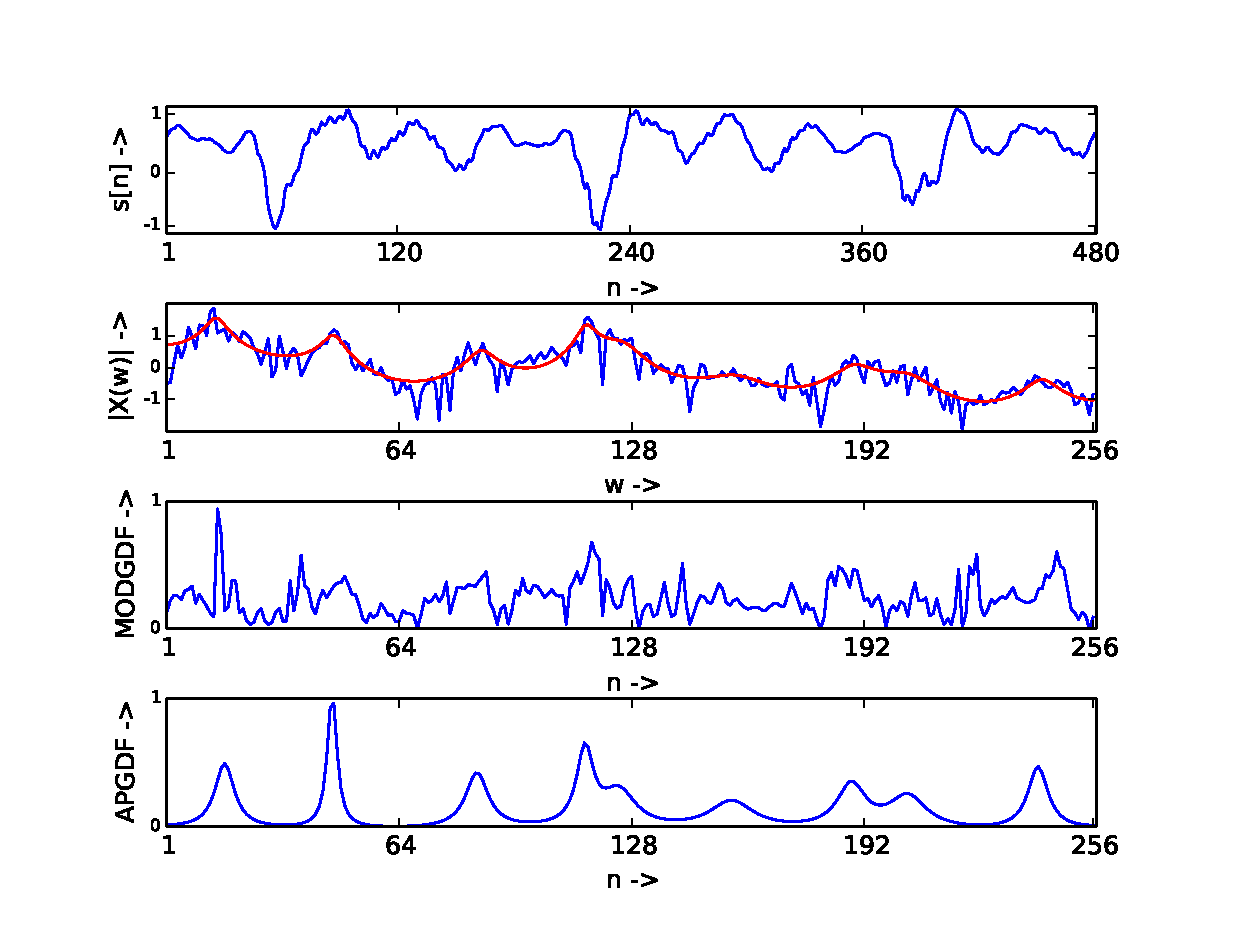
\includegraphics[width=0.5\textwidth]{figures/apSpectrum.eps}
\caption{A speech frame (in the top panel) with its Fourier spectrum(DFT) and spectrum approximation by all-pole model (in the bottom panel).}
\label{fig:all-pole}
\end{figure}
%\end{comment}

Number of the clusters is decided based on empirically determined threshold on Normalized mutual information(NMI) $\frac{I(Y,C)}{I(Y,X)}$. NMI is the fraction of information preserved in clustering representation $C$ about $Y$, out of the total amount of information contained in $X$ about relevance variables $Y$. As NMI decreases monotonically with number of clusters, and decrease in the value is expected to be higher when more dissimilar clusters (possibly belonging to different speakers) start merging. To apply the aforementioned method to diarization, one has to define $X = {x_i}$, i.e., set of input variables and $Y = {y_j}$ i.e. relevance variables. $X$ is constructed as a set of fixed length speech segments, typically for $2.5$ seconds based on output of voice activity detector. These segments are characterized by a background Gaussian mixture model(GMM) with shared diagonal covariance matrix and all components of GMM consist the set of relevance variables, i.e, $Y$. And the posteriors of each Gaussian component conditioned on speech segments, i.e., $p(y_j|x_i)$ computed using Bayes' rule. After clustering, further initially created speaker boundaries are refined using Viterbi realignment.

\subsection{Feature Analysis : MFCC v/s Group-delay based features}

In order to show the effectiveness of group-delay based features, i.e., MODGDF and APGDF, we measure Kullback-Leibler (KL) divergence on speech segments, i.e. $X={x_i}$ created to initiate the aIB clustering algorithm. All choose two speech segments among all available segments with in a speech recordings, are divided into inter-speaker and intra-speaker pairs, based on ground-truth of speakers. We computed mean and variance of KL divergence for both intra-speaker and inter-speaker pairs, as depicted in Table.\ref{table:kl-div}. For this task, we select $20$ recordings of different meetings from the entire available AMI meeting corpus used in our experiments. 


\begin{table}[h]
\centering

\label{table:kl-div}
\begin{tabular}{|l|l|l|}
\hline
Feature 			& Intra-speaker 			& Inter-speaker 	 \\ \hline
MFCC          			& 6.7/10.1               & 8.3/11.4       \\ \hline
MODGDF        			& 6.1/9.7                & 8.4/12.7       \\ \hline
APGDF         			& 5.5/9.7                & 8.6/11.9        \\ \hline
\end{tabular}

\vspace{0.4cm}
\caption{KL divergence for both inter-speaker and intra-speaker speech segments created at to initialize the aIB clustering algorithm.}
\end{table}

As it is clearly evident from the results in Table \ref{table:kl-div}, the mean and variance of KL divergence values of intra-speaker and inter-speaker are decreased and increased for both MODGDF and APGDF respectively. Mean and variance of KL divergence for intra-speaker has decreased which potentially indicates the discriminative power of MODGDF and APGDF for speaker information in the IB framework. Additionally, one must also notice that mean and variance of KL divergence for inter-speaker has also slightly increased for MODGDF and APGDF, which further adds on to show their ability to hold speaker information for IB framework based diarization.  

\subsection{Feature fusion : MFCC with Group-delay based features}

The IB based diarization system can be easily extended to fuse multiple features. For each feature stream, we learn a separate GMM with equal number of components and every component is aligned with speech segment used to initiate aIB. This enforces unique relationship among the learned GMM for different feature streams. In other words, if $\lbrace F_1,F_2,...,F_N \rbrace$ are the features to fuse, where $N$ is the number of features, than corresponding background model will have components $\lbrace M^{F_{1}},M^{F_{2}},...,M^{F_{N}}\rbrace$ corresponding to every feature stream. And the distribution for $p(y|x)$ can be computed as follows:       

\begin{equation}
p(y|x) = \sum _{i=1}^{N} W_i \times p(y|x^{F_{i}},M^{F_{i}})
\label{eq:feat_combs}
\end{equation}

One must notice that features are fused at the level of relevance variables, which allow to fuse probabilities instead of likelihoods, hence less affected by the number of dimensions of every feature stream (\cite{aIB}). Unfortunately, it introduces optimization of $W_i$ parameters, which is an computationally intensive task as for every new $W_i$ requires further optimization for parameters present in $p(y|x^{F_{i}},M^{F_{i}})$, e.g, $\beta$ of aIB.

%\begin{comment}
\begin{figure}[h]
\centering
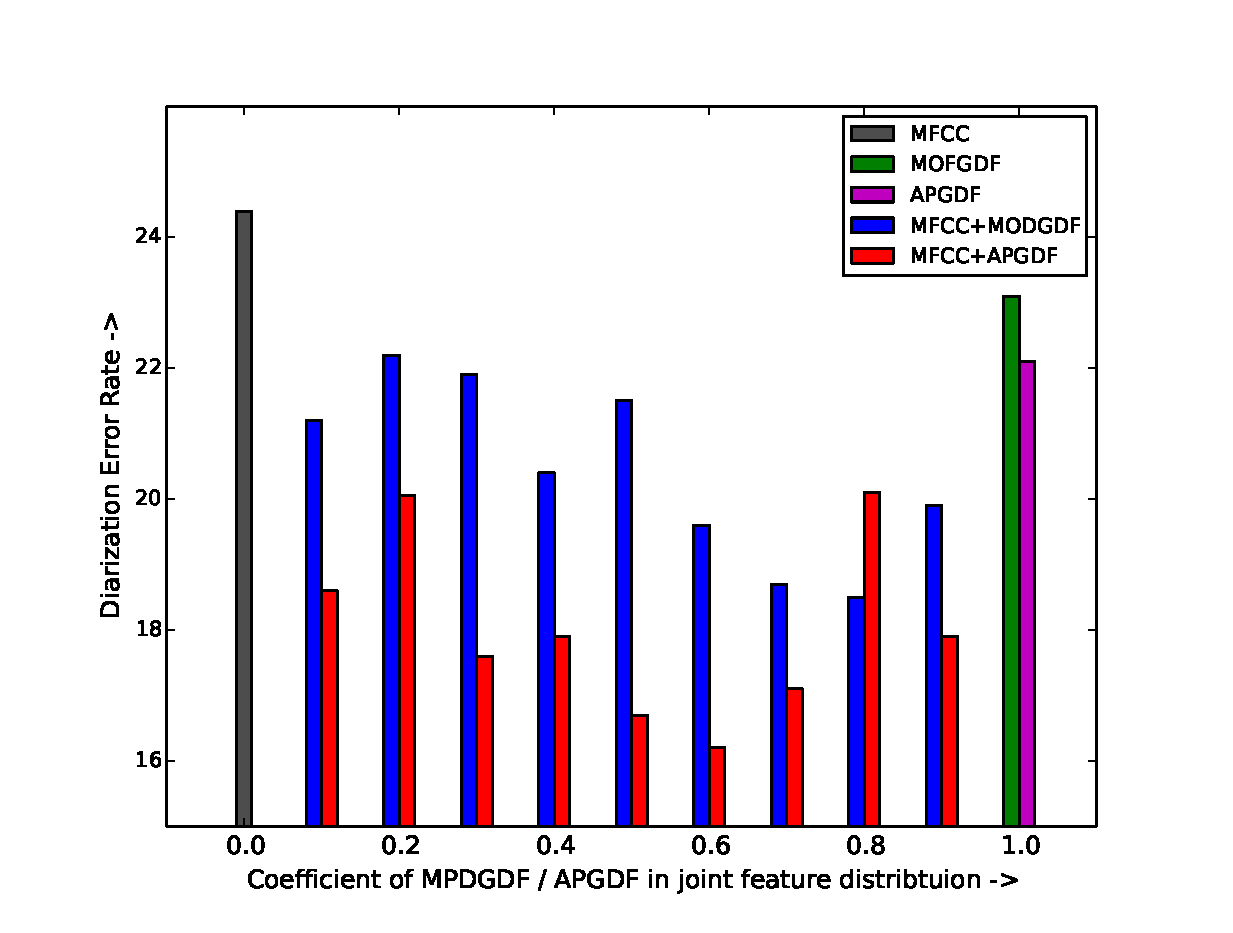
\includegraphics[width=0.5\textwidth,height=5.5cm]{figures/newFusionResults.eps}
\caption{Performance on AMI dataset comparing MFCC and its fusion with MODGDF and APGDF with respect to weight of probabilities used for MODGDF and APGDF features. Fusion weights are mentioned in parentheses.}
\label{fig:fusionResults}
\end{figure}
\end{comment}
Sum of all $W_i$ is bound to be $1$. Fig. \ref{intro} shows improvement in diarization error with increase in weight ($W_{MODGDF/APGDF}$) of probabilities arising from distribution of MODGDF and APGDF initially. Beyond a threshold, further increase in weight ($W_{MODGDF/APGDF}$) results in the deterioration of the performance as clearly visible in Fig. \ref{fig:fusionResults}.   

\section{Experiments and Results}
\label{experimentsNresults}

We evaluate the performance of the proposed group-delay based features for speaker diarization on publicly available AMI meeting corpus \cite{AMIData}. In our experiments, we select 100 meetings out of the total 170 meetings present in AMI corpus. Data is further divided into two parts, namely, development set consists of $30$ meetings and test set consists of remaining $70$ meetings. Optimal values of $\beta$ for aIB clustering and fusion weights (in case of feature fusion) are selected based on the performance on development set. Diarization error rate(DER) is used to measure the performance of various features. The definition of DER is as follows: 
\begin{equation}
DER = MISS + FA + SER
\end{equation}
\begin{comment}
\begin{equation}
	SER = \frac{\sum \limits_{s} {T_s ( min(N_{r}(s),N_{h}(s)) - N_{c}(s) ) } }  { \sum \limits_{s} T_s N_{r}(s)}
\end{equation}
\end{comment}

where MISS, FA and SER represents  missed speech errors, false alarm speech error, and speaker error (for details on DER see \cite{NIST}). In all the reported results, we have used the ground-truth speech/non-speech labels to drop non-speech segments of the meeting, which let DER indicate the speaker discriminative power more precisely. For optimization of fusion weights, we only look for $10$ values between $0$ and $1$ as shown in Fig. \ref{fig:fusionResults}.

%\begin{comment}
%\begin{figure}[h]
%\centering
%\includegraphics[width=0.5\textwidth,height=5.5cm]{Images/devNtest.png}
%\caption{Fusion results}
%\label{fig:fusionResults}
%\end{figure}
%\end{comment}

\subsection{Feature extraction using MODGDF and APGDF}

We perform frame-blocking with 50\%-overlapping windows of length 30 ms. Number of filters and length of feature vector for MFCC computation are $40$ and $18$ respectively. The procedure to compute MODGDF can be described below:

\begin{enumerate}
\item Compute discrete Fourier transform for speech frame $X[n]$ and its time multiplied version $Y[n]=nX[n]$.
\item Perform cepstrally smoothing on $|X(\omega)|$ to estimate $|S(\omega)|$ and plug it into Eg. \ref{eq:MODGDF} to obtain $\tau_{m}(\omega)$.
\end{enumerate}	
\vspace{0.2cm}
Procedure to compute APGDF can be described as follows:
\begin{enumerate}
\item Perform all-pole analysis(LP/WLP) on frame with prediction order set to $p=20$ and estimate values of coefficients $a(k)$ of all-pole filter.  
\item Use $G=1$ and $a(k)$ to compute frequency response $H(\omega)$ as defined in Eq. \ref{eq:homega}.
\item Now, group-delay function is computed by taking the negative derivative of the phase response of $H(\omega)$. Derivative is computed using sample-wise difference.
\end{enumerate}	
\vspace{0.2cm}
After computing MODGDF and APGDF, we perform discrete cosine transform and keep the first $18$ coefficients (excluding the zeroth one) in the feature representation. Additional parameters involved in MODGDF and APGDF ($\alpha = 0.9$, $\gamma=0.4$ and $p=20$) are picked from earlier studies done for speech and speaker recognition \cite{modifiedGD} and \cite{allPoleGdSid}. We omitting the search for the optimal value of the additional involved parameters due to two reasons: 1) As this task is highly computationally intensive experimentations, and 2) the fact that the primary motivation is to demonstrate whether group-delay based features are at all capable of improvement in the diarization systems. Search for optimal values to further refine the results is left for the future research.

%\begin{comment}
\begin{table}[h]
\centering
\label{my-label}
\begin{tabular}{|l|l|l|}
\hline
Feature Used  & Development Set & Test Set \\ \hline
MFCC          & 24.4                   & 26.3            \\ \hline
MODGDF        & 23.1                   & 25.1            \\ \hline
APGDF         & 22.1                   & 24.9            \\ \hline
MFCC + MODGDF(0.8,0.2) & 18.5          & 20.1            \\ \hline
MFCC + APGDF(0.6,0.4)  & 16.2          & 18.7            \\ \hline
\end{tabular}
\vspace{0.4cm}
\label{table:results}
\caption{Diarization error obtained on AMI dataset comparing various feature streams and their combinations. In case of fusion, optimum weights are mentioned in parentheses.}
\end{table}
%\end{comment}


\subsection{Results}

Table \ref{table:results} presents the results of various features and their combinations used for speaker diarization. Performance of MODGDF and APGDF fairly indicate that group-delay based features have the ability to represent speakers for IB based diarization system successfully. The relative improvements of $4.56\%$ and $4.56\%$ are obtained by MODGDF and APGDF with respect to MFCC respectively. Fusion of group-delay based features with MFCC has also been studied and the results of fusion experiments are reported for both MODGDF and APGDF as MFCC + MODGDF and MFCC + APGDF in Table \ref{table:results} respectively. The results indicate, as expected, the fusion of MFCC with group-delay based features have the potential to further push the performance up of the current diarization systems, as relative improvements of $23.5\%$ and $28.9\%$ for MFCC + MODGDF and MFCC + APGDF have been observed respectively.

Fusion weights for MFCC + MODGDF and MFCC + APGDF are found (0.8,0.2) and (0.6,0.2) respectively. We suspect relatively lesser improvements provided by MODGDF when compared to APGDF are due to omitted search process for parameters involved in its computation. Results show that performance of diarization system start improving on increase of the probability arising from the individually learned distribution of group-delay based features, as it is clearly evident from the Fig. \ref{fig:fusionResults}. Interestingly, we found there is always an improvement for any choice of fusion weight, when compared to both MFCC and group-delay based features standalone.     


\section{Conclusion And Future Work}
\label{conclude}
In this work, we investigated the use of group-delay based features in IB based diarization system. Using with and without model based techniques, namely, MODGDF and APGDF, to estimate group-delay function and used them further to derive features for diarization. We found that features derived from MODGDF and APGDF provide better diarization error rate. Furthermore, fusion with MFCC has yielded a significant improvement in the diarization accuracy.  In future, it will be particularly interesting to further investigate their performance in more complex scenarios, e.g., for overlapped speech and speech/non-speech detection at early stage of a diarization system. Additionally, fusion study of other spectral and time domain features with group-delay based features appears reasonable direction to explore further. 

\bibliographystyle{IEEEbib}
\bibliography{bare_conf}

\end{document}


